\chapter{Background}\label{chap:background}

This background section will explain some of the concepts, approaches, technologies and software architectures required to understand this thesis.
The findings from the pre-project in \cite{rekstadModelingEnvironmentCloud2020} will also be presented in more detail than the introduction, as the findings are central to this thesis.
Lastly, a section on open source software project management follows, as they shape many of the choices made in the implementation of a solution.

\section{Conceptual Modeling and Model-Driven Development}\label{sec:conceptual-modeling}

\paragraph{Rationale}
\Acrfull{MDD} is the approach to software development which this thesis aims to support.
Therefore, and understanding of \acrshort{MDD} is beneficial, in order to see how an editor should work.

\paragraph{Modeling and abstraction}
The core of \acrshort{MDD} is the model.
The model is a human created construct, formed through humans working together to discuss and refine a problem domain until they reach a consensus of what abstractions help them solve the relevant problems~\cite[p.~154]{brambillaModeldrivenSoftwareEngineering2012}.
Humans perceive the world (and problem domain) as many different phenomena, and conceptual modeling is the act of trying to describe these at some level of abstraction~\cite[p.~1,408]{krogstieModelbasedDevelopmentEvolution2012}.
The model is assumed to resemble the phenomena and work the same way, and yet be simpler than the real world~\cite[p.~414]{krogstieModelbasedDevelopmentEvolution2012}.
Abstraction means to find something common in different observations of a phenomena, and \textit{generalize} their features, \textit{classify} coherent clusters of objects and \textit{aggregate} concepts into more complex ones~\cite[p.~1]{brambillaModeldrivenSoftwareEngineering2012}.
The model will never describe every aspect of the world perfectly, but can \textit{reduce} the world down to relevant aspects, and easily \textit{map} between model elements and real world phenomena~\cite[p.~1-2]{brambillaModeldrivenSoftwareEngineering2012}.


\paragraph{Modeling languages}
In order to describe the model, a \textit{language} is used.
To realize the benefits of \acrshort{MDD}, a \textit{formal language} is used.
The language can be textual or graphical, or both, and imposes a formally defined syntax on the modeler~\cite[p.~13]{brambillaModeldrivenSoftwareEngineering2012}.

\paragraph{Modeling tools}
The advantage of using a formal language is that it can be parsed and understood by software tools, as well as humans.
The tools can validate the model according to the syntax, and to specific rules for the domain.
Tools can also generate code, or execute the model itself.
The model can be transformed into other models, or text or graphics~\cite[p.~8]{brambillaModeldrivenSoftwareEngineering2012}.

\paragraph{\acrlong{MDD}}
The central idea of \acrlong{MDD} is that the model is the source of truth that \textit{drives} the rest of the engineering and development~\cite[p.~9]{brambillaModeldrivenSoftwareEngineering2012}.
There is not a separate model for analysis and for design, but a single one for both~\cite[p.~49]{evansDomaindrivenDesignTackling2004}.
The software code becomes an expression of the model itself, and changes to the code often happen as the result of changes to the model~\cite[p.~49]{evansDomaindrivenDesignTackling2004}.
Because the model and the software are so directly related, the \acrshort{MDD} approach is heavily reliant on tools to automate the tasks of validation and code generation.
The formal language may also sacrifice some of its human readability in order to be understood by tools~\cite[p.~232]{krogstieModelbasedDevelopmentEvolution2012}.
To solve this, one can use other tools that interpret, transform or present models in other ways~\cite[p.~233]{krogstieModelbasedDevelopmentEvolution2012}.
This increases the reliance on tools for \acrshort{MDD} even more, including visual editors.




\section{Model-Driven Development at NTNU in the Course TDT4250}\label{sec:tdt4250}
% * TDT4250. Modeling, use of instances to validate model as you develop, validation of models.

\paragraph{Rationale}
Because the target audience of the software solution (tree editor) are students at \acrshort{NTNU}, it is helpful to know how they work with \acrlong{MDD}.
Their use cases are the ones being solved, meaning the solution must be made with this context in mind.

\paragraph{\Acrshort{MDD} at \acrshort{NTNU}}
To do \acrlong{MDD} effectively, tools should be used.
In the course ``\textit{\gls{TDT4250} Advanced Software Design}''\footnote{Course description is available at \href{https://www.ntnu.edu/studies/courses/TDT4250\#tab=omEmnet}{https://www.ntnu.edu/studies/courses/TDT4250\#tab=omEmnet}.} at \acrshort{NTNU}, the chosen tools are in the \acrfull{EMF}~\cite{hallvardtraettebergEMFTDT4250NTNU2017}.
This includes the modeling language \gls{Ecore}, visual editors in \gls{Eclipse}, model validation logic, the code generator named ``GenModel''\footnote{The code generator is actually named ``codegen'', but users only see the configuration model called ``GenModel''.} (generator model), and more.
\Acrshort{EMF} is a battle-tested technology also used in certain industries, and is well integrated with the \gls{Eclipse}.
The course \gls{TDT4250} also uses \gls{Eclipse} as a case study for other software design concepts, such as modularity (plugin architecture) and dynamic systems (OSGi), and custom \acrlongpl{DSL} which automatically work with \gls{Eclipse}.
\Acrshort{EMF} is relevant for most or all of those concepts.

\paragraph{Development methodology}\label{par:tdt4250-methodology}
Students are taught a methodology or approach for how to do modeling.
They start by specifying a problem space, for example bookkeeping an organization of employees or the courses in \acrshort{NTNU}, and then abstract the problem into a model.
The initial model is externalized as \gls{Ecore} by using a tree editor in \gls{Eclipse}.


Then an \textit{model instance} is made, based on the model, and filled with example data from the domain.
This model instance is used to test and verify that the model is appropriate for the problem space.
Adjustments are made to the model to accommodate any problems with the model instance.


Then validations can be created for the model, by one or both of the following approaches: writing \acrfull{OCL} into model annotations, or marking the model element with an annotation and implementing it as java code.
\Acrshort{OCL} is a \acrlong{DSL} for navigating models and evaluating expressions, and the \gls{Eclipse} can detect annotations with \acrshort{OCL} and evaluate them against the \gls{Ecore} model.
The other option, writing java code, requires the student to first create a new \textit{genmodel} file from the model (by using a menu in \gls{Eclipse}), generating a java code project from the model, and then writing validation logic into the generated code.
For the java code to be picked up, \gls{Eclipse} can start a new instance which installs the generated code as a plugin~\cite{hallvardtraettebergConstraintsValidationTDT42502020}.


Next up, when the model is deemed sufficient, and the most important validations are in place, the student can try to create a user interface.
One of several choices here is to create an \textit{\gls{Eclipse} plugin}.
\Acrshort{EMF} provides code generation for utilities used to integrate the model into an editor for \gls{Eclipse}.
The student uses the genmodel to create these, and tweaks the code if wanted.
Then everything is installed into \gls{Eclipse} by launching a new \gls{Eclipse} instance with the code installed as a plugin.


Lastly, the user interface can be tested.
The student creates a new model instance file, enters some example data from the domain, and runs validation logic.

\paragraph{Lecture materials}\label{par:tdt4250-confluence}
The steps mentioned in the methodology above are available online in \cite{hallvardtraettebergEMFStepbystepTDT42502017,hallvardtraettebergConstraintsValidationTDT42502020,hallvardtraettebergEditingEcoreModel2017,hallvardtraettebergGenmodelTDT4250NTNU2017}.
This is an advantage, because they can by used used in this master's thesis as a basis for creating evaluations and acceptance criteria.



\section{Eclipse Modeling Framework Editors for Ecore}\label{sec:emf-editors}

\paragraph{Rationale}
These editors are the ones being re-implemented in \gls{cloud}-based \acrshortpl{IDE}.
Understanding their functionality and workings is important, as these editors shape the work of this thesis.
The functionalities provided are assumed highly usable and good, because they are the result of many years of work and experience.
This allows this thesis to skip the work of doing usability testing with regards to feature design, as long as the features are similar enough to the copied ones.

\paragraph{Multiple editors}
When editing \gls{Ecore} models in \gls{Eclipse}, there are different editors to pick from.
Usually, \gls{Ecore} models and model instances are saved as \acrfull{XMI}, which is a standardized serialization format based on XML.
The \gls{Ecore} models have the file extension \texttt{.ecore} while model instances either have \texttt{.xmi} or a custom extension for the model, specified by the modeler (e.g. \texttt{.organization} or \texttt{.courses}).
The GenModel has \texttt{.genmodel} as file extension.
However, \gls{Ecore} models are rarely (if ever) edited as XML.
Instead, the files are loaded and presented in a tree structure editor or diagram editor.
These editors are specialized for \gls{Ecore}, and can understand the model.


The diagram based editors use a notation that is based on \gls{UML} Class Diagrams, with boxes, labels and arrows.
Which editor to use can often be a personal preference.
They are all functionally equivalent, with regards to modeling.
The next subsections will describe the most common tree editors in more detail.

\subsection{Sample Reflective Ecore Model Editor}\label{sec:sample-reflective-editor}

The ``\textit{Sample Reflective Ecore Model Editor}'' is one of the main \gls{Ecore} editors in \gls{Eclipse}.
A screenshot of the editor is shown in \cref{fig:sample-reflective-ecore-model}.
The model instances can be edited in a \textit{reflective} editor (without the user first generating java code and installing an \gls{Eclipse} plugin).
Here, reflective means that the editor uses a metamodel (see \cref{sec:emf-metamodel}) for the model instance, and tries to infer the tree structure from containment relationships.


This editor can open both \gls{Ecore} models and model instances.
A screenshot of a model opened in the editor is shown in \cref{sfig:sample-reflective-ecore-model-screenshot}, and a model instance in \cref{sfig:sample-reflective-ecore-model-instance-screenshot}.


This editor is \gls{open source}%
\footnote{Sample Reflective editor source: \href{https://git.eclipse.org/c/emf/org.eclipse.emf.git/tree/plugins/org.eclipse.emf.ecore.editor}{\nolinkurl{https://git.eclipse.org/c/emf/org.eclipse.emf.git/tree/plugins/org.eclipse.emf.ecore.editor}}.}%
, and the editor is itself originally generated by a genmodel~\cite[p.~10]{rekstadModelingEnvironmentCloud2020}.


This editor internally uses a java class called \texttt{ReflectiveItemProvider}%
\footnote{\texttt{ReflectiveItemProvider} source code: \href{https://git.eclipse.org/c/emf/org.eclipse.emf.git/tree/plugins/org.eclipse.emf.edit/src/org/eclipse/emf/edit/provider/ReflectiveItemProvider.java}{\nolinkurl{https://git.eclipse.org/c/emf/org.eclipse.emf.git/tree/plugins/org.eclipse.emf.edit/src/org/eclipse/emf/edit/provider/ReflectiveItemProvider.java}}}
from the \texttt{org.eclipse.emf.edit} \acrshort{EMF} package, to extract text labels and infer icons for the tree view~\cite[p.~10]{rekstadModelingEnvironmentCloud2020}.


For \gls{Ecore} models (with \texttt{.ecore} file extension, not model instances), it uses an \texttt{EcoreItemProviderAdapterFactory}%
\footnote{\texttt{EcoreItemProviderAdapterFactory} source code: \href{https://git.eclipse.org/c/emf/org.eclipse.emf.git/tree/plugins/org.eclipse.emf.ecore.edit/src/org/eclipse/emf/ecore/provider/EcoreItemProviderAdapterFactory.java}{\nolinkurl{https://git.eclipse.org/c/emf/org.eclipse.emf.git/tree/plugins/org.eclipse.emf.ecore.edit/src/org/eclipse/emf/ecore/provider/EcoreItemProviderAdapterFactory.java}}}
to get labels and icons~\cite{edmerksEcoreEditorJava2021}.


These ``item providers'' are especially interesting, because they could be reused in a new editor.

\begin{figure}
    \centering
    \begin{subfigure}[b]{.45\textwidth}
        \centering
        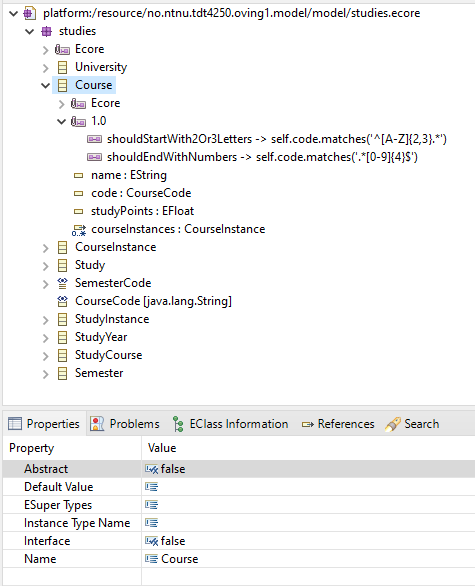
\includegraphics[width=\textwidth]{figures/pre-project/ecore-sample-reflective-ecore-model-editor}
        \caption{A model opened in the editor.}\label{sfig:sample-reflective-ecore-model-screenshot}
    \end{subfigure}
    \hfill
    \begin{subfigure}[b]{.45\textwidth}
        \centering
        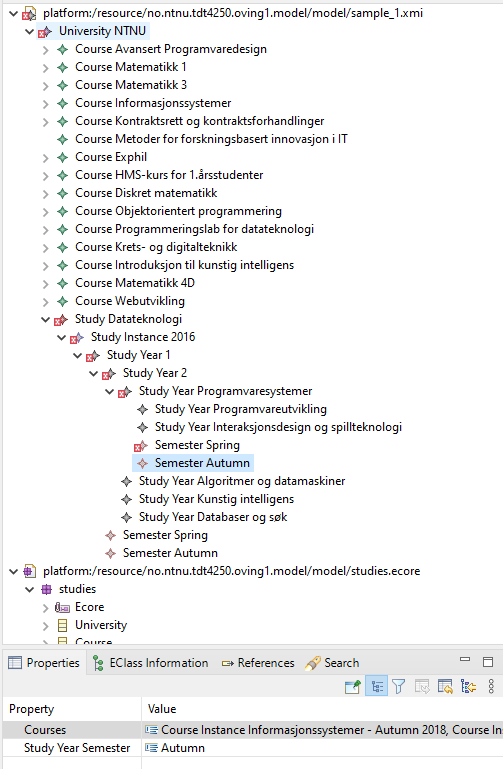
\includegraphics[width=\textwidth]{figures/pre-project/ecore-sample-reflective-ecore-model-editor-instance.png}
        \caption{A \emph{dynamic instance} (\acrshort{XMI} file) opened in the editor.}\label{sfig:sample-reflective-ecore-model-instance-screenshot}
    \end{subfigure}
    \caption{Screenshots of the Sample Reflective Ecore Model Editor in \gls{Eclipse}.}\label{fig:sample-reflective-ecore-model}
\end{figure}


\subsection{EMF Forms Ecore Editor}\label{sec:emfforms-editor}

The \textit{EMF Forms Ecore Editor} is a newer editor than the Sample Reflective editor, and uses EMF Forms\footnote{More info about EMF Forms here: \href{https://www.eclipse.org/ecp/emfforms/index.html}{\nolinkurl{https://www.eclipse.org/ecp/emfforms/index.html}}.} as the technology to provide a user interface~\cite{eclipsesourceEMFFormsEditors2016}.
This editor is \gls{open source}%
\footnote{\textit{EMF Forms} source code: \href{https://git.eclipse.org/c/emfclient/org.eclipse.emf.ecp.core.git/tree/bundles/org.eclipse.emfforms.editor.ecore}{\nolinkurl{https://git.eclipse.org/c/emfclient/org.eclipse.emf.ecp.core.git/tree/bundles/org.eclipse.emfforms.editor.ecore}}.}.
A screenshot of the editor is shown in \cref{fig:emf-forms-ecore-editor}.


This editor is implemented as a generic editor for all \gls{Ecore} model instances, and two subclasses that are specialized for \gls{Ecore} and GenModel~\cite{eclipsesourceEMFFormsEditors2016}.
The generic editor is called \textit{Generic XMI Editor} in \gls{Eclipse}, and the \gls{Ecore} specific editor is called \textit{Ecore Editor}.


The biggest difference compared to the Sample Reflective editor, is how the user interface looks, and that the property sheet is customized based on a \textit{view model file}.
The Sample Reflective editor uses \gls{Eclipse}'s built in property panel.
In the EMF Forms editor, the properties are also grouped into \textit{standard} and \textit{advanced}.

\begin{figure}[htbp]  % order of priority: h here, t top, b bottom, p page
  \centering
  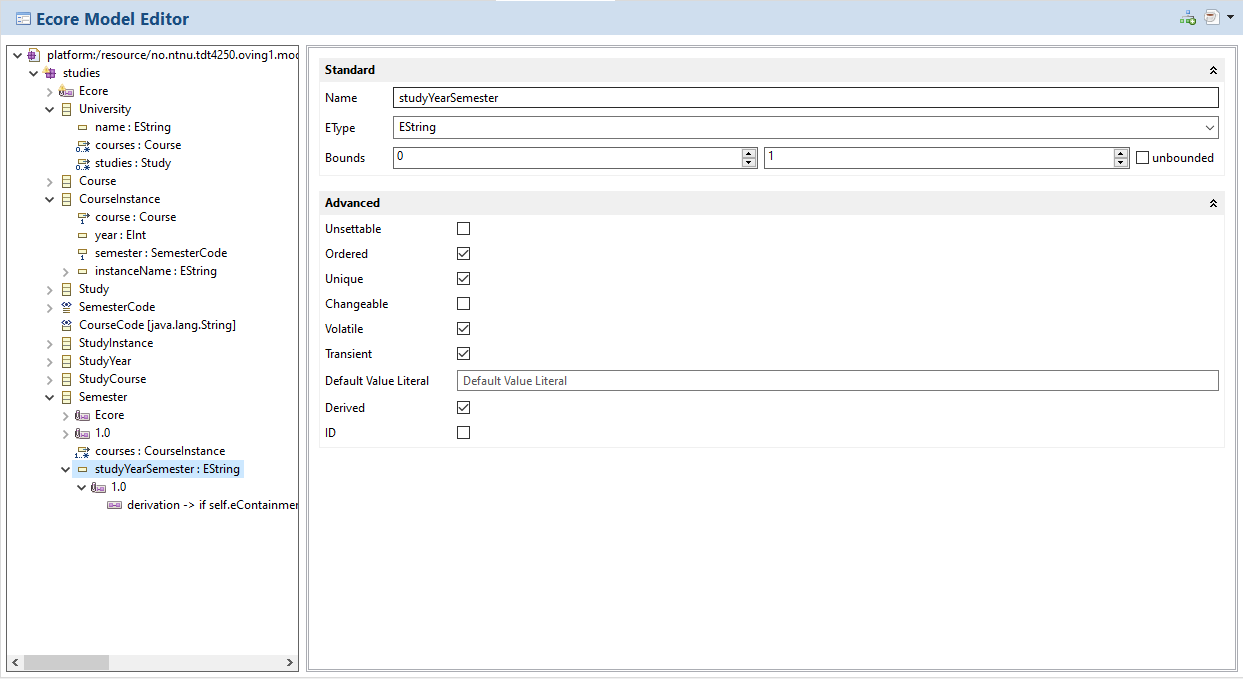
\includegraphics[width=\textwidth]{figures/pre-project/ecore-eclipse-emf-forms-model-editor.png}
  \caption[EMF Forms Ecore Editor]{A screenshot of a model in the EMF Forms based Ecore Editor.}\label{fig:emf-forms-ecore-editor}
\end{figure}

\iffalse{} 
{
%Skip diagrams for now. Tree editors are more important.

  \subsection{Ecore Tools diagrammatical editor}\label{sec:ecore-tools-editor}
  
  The \textit{Ecore Tools} editor presents \gls{Ecore} as class diagrams, similar to \gls{UML} Class Diagrams.
  
  \subsection{EMF.Cloud ecore-glsp diagrammatical editor}\label{sec:ecore-glsp-editor}
  %TODO
  
}
\fi


%* Eclipse EMF offers different Ecore editors. Tree-editor is important for developers, and diagrams are important in runtime and end-users.



\section{Introduction to Tree Structures}\label{sec:tree-structures}

\paragraph{Rationale}
Because the editors center around a tree structure, a clear understanding of trees is helpful.

\paragraph{Trees}
A \textit{tree} is a data structure.
The tree is composed of \textit{nodes}, and one node is designated as the \textit{root node} node or \textit{tree root}.
Each node can have zero or more \textit{children} nodes, and one \textit{parent} node.
The root node does not have a parent.
When representing the tree as code, it is possible to omit either the parent or child relationship in a node, making the parent or child implicit.
The relationship can still be found, by \textit{traversing} the tree.
Traversing means to visit every node it the tree by following the parent or child relationships.


\paragraph{Visualizing trees}
There are many ways to present trees to humans.
Two common approaches are \textit{hierarchy} and \textit{diagram}.


In a hierarchy, the parent is presented as a row, and its children on separate rows below (see \cref{sfig:tree-visualized-hierarchy}).
The children are often indented as well, and possibly connected with dots or lines to the parent.


In a diagram, nodes are often displayed as a circle or box (see \cref{sfig:tree-visualized-diagram}).
The parent is displayed above its children, and the children are aligned on the same row.
The parent-child relationship is shown as a line or arrow, connecting the parent to the child.

\begin{figure}[htbp]
    \centering
    \begin{subfigure}[b]{.45\textwidth}
        \centering
        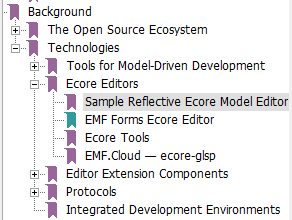
\includegraphics[width=\textwidth]{figures/tree-hierarchy.png}
        \caption{A tree visualized as a hierarchy. The top node is the root.}\label{sfig:tree-visualized-hierarchy}
    \end{subfigure}
    \hfill
    \begin{subfigure}[b]{.45\textwidth}
        \centering
        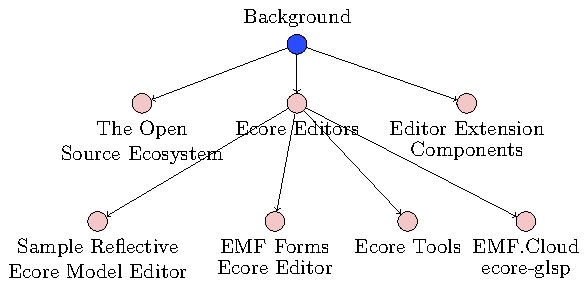
\includegraphics[width=\textwidth]{figures/tree-diagram.pdf}
        \caption{A tree visualized as a diagram. The blue node at the top is the root.}\label{sfig:tree-visualized-diagram}
    \end{subfigure}
    \caption{A tree visualized as a hierarchy and diagram. The labels are section titles of \cite{rekstadModelingEnvironmentCloud2020}, as an example.}\label{fig:tree-visualized}
\end{figure}

\paragraph{Nodes}
The tree is more useful when the nodes have properties.
The minimum property is children or parent.
But a useful property is a name, label or id, with regards to presenting the tree to a human.
There may be properties on the relationships between a node and its children, but these may be hard to present visually in hierarchy-type visualizations.
For a diagram type visualization, the properties may be presented as labels on the edge.

\paragraph{Mapping to trees}
A data structure can be mapped to a tree if it has separate objects with a containment or aggregation relationship.
There can be different ways to map to a tree, depending on what properties are used (or not used).
The labels can also come from various object properties, be derived from them or combine multiple properties into one label.



\section{Master-Detail Tree Editor}\label{sec:master-detail}

\paragraph{Rationale}
The tree editors use a layout pattern called \textit{master-detail}.

\paragraph{Description}
As the name \textit{Tree Editor} implies, they are used to edit a tree.
There are mainly two different things that can be edited: the parent-child relationships and the node's properties.
The user interfaces for the tree editors in \cref{sec:emf-editors} use a pattern called \textit{master-detail}.
This means the user interface is composed of two parts: a \textit{master view} and a \textit{detail view}.
% TODO: add a figure of master-detail overlayed on an editor?


\paragraph{Master view}
The tree structure is shown as a hierarchy in the master view.
It is common for the master view to be positioned to the left of a detail view, or above it.
The user interacts with the master view to add, remove and select nodes.
Adding a new child to a parent is done here.


\paragraph{Detail view}
When a node is selected, its properties are displayed in the detail view.
It is common for the detail view to be positioned to the right of a master view, or below it.
The detail view is usually a \textit{input form} or tabular (rows and cells) structure.
The user usually enters text, numbers, ticks checkboxes and opens selection dialogues from the detail view.


\section{The Eclipse Reflective Ecore Editor}

* Reflective Ecore Editor, its architecture, Commands in .Edit, works on any model.
% TODO: remove? DUplicate of prev. section?

\section{An Overview of EMF:\ Ecore Metamodel, XMI Serialization and GenModel for Code Generation}\label{sec:emf-metamodel}

\paragraph{Rationale}

\paragraph{\acrlong{EMF}}
% eclipse editor plugins, language, codegen, ocl, serialization format

\paragraph{Ecore metamodel}
% Class, package, attribute, reference

\paragraph{\Acrshort{XMI} serialization}
% serialization, standardized EMOF, default for ecore, XML,

\paragraph{Ecore java \acrshort{API}}
% EPackage registration, instance, factory, EList, EditingDomain, ItemProvider, Resource and ResourceSet

\paragraph{GenModel code generation}
% Template based, configuration options, model + .edit + .editor output

\paragraph{Custom code}
% editing genmodel code. @generated NOT annotation


* Ecore metamodel, EMF, XMI, genmodel. Adaptation of editors to special cases like Ecore model and Genmodel.

\section{Visual Studio Code's Custom Editor API}

* VSCode Custom Editor API enables any type of graphical editor to be made, not just text.

\section{Language Server Protocol Architecture}

* LSP from VSCode solves language-to-editor m*n combinations. There is already a need to move EMF from Eclipse to VSCode, it might need to move to IntelliJ etc. in the future.

\section{\acrlong{EMF} in the \Gls{cloud}}

* Recent development, EMF.Cloud Model Server, EMF.Cloud EMFJson, GLSP, GLSP Ecore Editor, GLSP Coffee Editor.

\section{Pre-project Findings about Architecture and Protocol for a Solution}

* The pre-project suggested an architecture for a VSCode Extension based on LSP. It confirmed the feasibility of the client-server model with a custom editor, the major blockers for this architecture.
  * It also suggested a data structure for general purpose tree editing.
  * It suggested a base protocol on which to build the TLSP on, but did not implement it.

\section{Pre-project Findings about Software Requirements}

* Non-functional requirements from empirical evidence, to increase the chance of project adoption of the Eclipse ecosystem.
    * Flexibility - customize rendering and logic for different models.
    * Configurability - alter or toggle behavior per-project based on config files.
    * Conforming to existing architectures that are empirically validated, and familiar to the Eclipse ecosystem developers.

* Functional requirements were extracted in pre-project from Eclipse IDE's EMF tree editors.
  * View models of different levels, from Ecore metamodel to model instances.
  * View model as a tree based on containment properties.
  * Create empty model files with the minimum file contents.
  * Edit model hierarchies by creating, deleting or moving tree nodes.
  * Edit tree node properties by using a form-based editor.
  * Saving model changes to xmi files.
  * Validation of models.
  * Generation of code from models.


\section{Open Source Software Project Management and Project Viability}

* What can make this Open Source software project viable and worth pursuing further? Anecdotal and empirical evidence, not research.
  * This project needs to live on after the delivery of the Thesis.
  * Correct open source licenses, and "licence hygience" wrt. copy-pasting. Eclipse Foundation do thorough licence reviews.
  * Use of programming languages accepted by the developer community.
  * Use of automated build systems accepted by the developer community.
  * Testable code to reduce legacy and maintenance burden.
  * Human readable, clean code. Correct use of Design Patterns. Clean separation of concerns.
  * Use of commonly used and recognized dependencies/libraries/frameworks/tools.
  * CI/CD.
  * Good developer documentation. Architecture diagrams. Informative Readme-files with pictures of the running software. Instructions for developer environment setup.
  * Google Design Documents (?). Not too common in this ecosystem, but valuable inside Google. Complements the readme.
  * Publicly available bug/issue tracker and roadmap.
  * Release management. Semantic versioning. Changelogs. More useful for end-users or those using this as a library/dependency.
  * Specific to Eclipse Foundation, is the "Eclipse Foundation Project Handbook" (https://www.eclipse.org/projects/handbook/) and its checklist.
  * Measures to reduce new-developer onboarding and friction.
